\documentclass{exam}
\usepackage{graphicx} 


%Format Header and footer
\pagestyle{headandfoot}
\header{\footnotesize Klass:\\Namn:}{\Large\textbf{Celldelning och mutationer}}{\footnotesize  BIOBIO01 - 2023\\Viktor Arohlén}
\headrule
\footrule
\setlength{\columnsep}{0.25cm}
%\setlength{\columnseprule}{1pt}
\footer{}{Sida \thepage}{}
%\extrafootheight{-2cm}

\begin{document}
\vspace{5mm} %5mm vertical space
\begin{center}
\fbox{\fbox{\parbox{6in}{\centering
\textbf{10 kryssfrågor}: markera endast ett alternativ. (1 poäng per fråga.)
}}}
\end{center}
\vspace{5mm} %5mm vertical space

\begin{questions}

\question Skillnaden mellan \textbf{kromatin} och \textbf{DNA} är:
\begin{checkboxes}
   \choice Kromatin är DNA och de hjälpproteiner som är involverade i packningen av DNA
   \choice Det är ingen skillnad
   \choice DNA är endast i människan, kromatin syftar på alla andra arter
   \choice Kromatin är namnet på hjälpproteiner, medan DNA är den genetiska koden
\end{checkboxes} 

\vspace{5mm} %5mm vertical space
\hrule 
\vspace{5mm} %5mm vertical space

\question Hur många \textbf{kromosomer} har en människa?
\begin{checkboxes}
   \choice 23
   \choice 46
   \choice 47
   \choice 92
\end{checkboxes} 



\vspace{5mm} %5mm vertical space
\hrule 
\vspace{5mm} %5mm vertical space
\question När sker \textbf{överkorsning}?
\begin{checkboxes}
   \choice Profas I
   \choice Profas II
   \choice Metafas II
   \choice Anafas I
\end{checkboxes}

\vspace{5mm} %5mm vertical space
\hrule 
\vspace{5mm} %5mm vertical space
\question Vad är slutresultatet i \textbf{meiosen}? 
\begin{checkboxes}
   \choice Två diploida celler
   \choice Två haploida celler
   \choice Fyra diploida celler
   \choice Fyra haploida celler
\end{checkboxes}

\vspace{5mm} %5mm vertical space
\hrule 
\vspace{5mm} %5mm vertical space
\question Vad av följande kan \textit{inte} öka risken för en skadlig \textbf{mutation}?
\begin{checkboxes}
   \choice Utsättas för radioaktiv strålning
   \choice Rökning
   \choice Giftiga kemikalier i för hög dos
   \choice Dricka 4 liter vatten om dagen
\end{checkboxes}
\break

\question I vilken organell hittar vi \textit{inte} \textbf{DNA} eller \textbf{RNA}?
\begin{checkboxes}
   \choice Cellkärna
   \choice Mitokondrie
   \choice Ribosom
   \choice Cellmembran
\end{checkboxes}
\vspace{5mm} %5mm vertical space
\hrule 
\vspace{5mm} %5mm vertical space
\question Vad krävs för att en \textbf{mutation} ska vara ärftlig? 
\begin{checkboxes}
   \choice behöver undvika cellens reparationsmekanismer
   \choice behöver ske fler än en gång
   \choice behöver ske i en könscell
   \choice behöver ske hos ett embryo (foster)
\end{checkboxes}

\vspace{5mm} %5mm vertical space
\hrule 
\vspace{5mm} %5mm vertical space
\question En \textbf{gen} är:  
\begin{checkboxes}
   \choice ett annat namn för DNA
   \choice en typ av RNA
   \choice en modell för hur egenskaper ärvs
   \choice ett DNA-segment som kodar för ett specifikt protein
\end{checkboxes}

\vspace{5mm} %5mm vertical space
\hrule 
\vspace{5mm} %5mm vertical space
\question  Vad sker i \textbf{interfasen} och är viktigt för celldelningen?
\begin{checkboxes}
   \choice Transkription
   \choice Translation
   \choice Profas
   \choice Replikation
\end{checkboxes}


\vspace{5mm} %5mm vertical space
\hrule 
\vspace{5mm} %5mm vertical space
\question  Vad innebär en \textbf{trisomi}?
\begin{checkboxes}
   \choice En typ av genmutation
   \choice En extra kromsom i ett av det mänskliga genomets kromosompar
   \choice Avsaknad av en del av en kromosom
   \choice En infektionssjukdom orskad av bakterier
\end{checkboxes}
\break



\vspace{5mm} %5mm vertical space
\begin{center}
\fbox{\fbox{\parbox{6in}{\centering
\textbf{4 kortsvarsfrågor}: Svara kortfattat på utrymmet under frågan. Använd relevanta begrepp och figurer. (2 poäng per fråga)
}}}
\end{center}
\vspace{5mm} %5mm vertical space
\question Matcha vad som händer i \textbf{mitosen} med rätt fas (\textit{OBS!} Det kan vara flera händelser i en fas.) 

\begin{tabular}{p{0.45\textwidth}p{0.45\textwidth}}
  \begin{minipage}[t]{\linewidth}
    \begin{itemize}
      \item[\textbf{A.}] Systerkromatider organiserar sig längs cellens mittlinje.
      \item[\textbf{B.}] Kromatinet packas ihop i två separata kärnor.
      \item[\textbf{C.}] Kärnmembranet är helt upplöst.
      \item[\textbf{D.}] Kromosomer börjar bli synliga genom att kromatinet kondenseras
    \end{itemize}
  \end{minipage}
  &
  \begin{minipage}[t]{\linewidth}
    \begin{itemize}
      \item[\textbf{1.}] Profas
      \item[\textbf{2.}] Metafas
      \item[\textbf{3.}] Anafas
      \item[\textbf{4.}] Telofas
    \end{itemize}
  \end{minipage}
\end{tabular}
\question 
\vspace{10mm} %5mm vertical space
Hur är \textbf{DNA} organiserat i \textbf{cellkärnan}? Varför ser det ut så? 
\vspace{40mm} %5mm vertical space
\question 
Hur kommer det sig att en \textbf{genmutation} ibland inte påverkar genuttrycket? Ge exempel
\vspace{40mm} %5mm vertical space
\question 
Vad är skillnaden på en \textbf{malign}- och en \textbf{benign} tumör?

\break
\vspace{5mm} %5mm vertical space
\begin{center}
\fbox{\fbox{\parbox{6in}{\centering
\textbf{4 frisvarsfrågor}:  Svara på utrymmet under frågan. Anvönd relevanta begrepp och figurer. (3 poäng per fråga)
}}}
\end{center}
\vspace{5mm} %5mm vertical space

\question 
Varför är \textbf{meios} den primära celldelningen vid förökning hos flercelliga arter? Vad är för- och nackdelarna?
\vspace{80mm} %5mm vertical space
\question 
2015 fick tre stycken forskare (Tomas Lindahl, Paul Modrich, och Aziz Sancar) Nobelpriset i Kemi för följande upptäckter: \textit{ base excision repair}, \textit{mismatch repair}, och \textit{nucleotide excision repair}. 
\\ \\
Utifrån dina kunskaper och tolkning av ovan, vad har upptäckterna för betydelse kopplat till \textbf{celldelning}, \textbf{mutationer}, och \textbf{cancer}? 
\vspace{60mm}

\break

\question
\textbf{Downs syndrom} är ett exempel på en kromsomavvikelse. Vid denna typ av avvikelse kan individen leva ett relativt normalt liv och uppnå vuxen ålder. Vad händer vid de flesta kromosomavvikelser och varför? Varför skiljer det sig vid Down's syndrom? 
\vspace{70mm}


\question
En mänsklig spermie är miljontals gånger mindre än en mänsklig äggcell. Vad kan det ha för fördelar och nackdelar med så olika storlek på könscellerna utifrån dina kunskaper om celldelning och förökning? 
\\ \\ \\
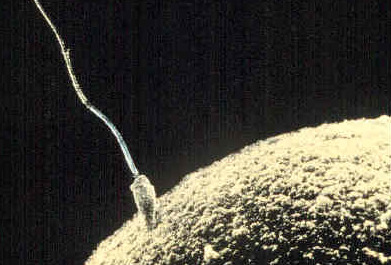
\includegraphics[width=3 cm]{Sperm-egg.jpg}





\end{questions}





\end{document}
